\section{Compartmental model fit validation}
\label{appendix:compartmentalModelFitValidation}
%\subsection{T$_{Hill}$IRVV$_i$}

\begin{figure}[H]
\begin{center}
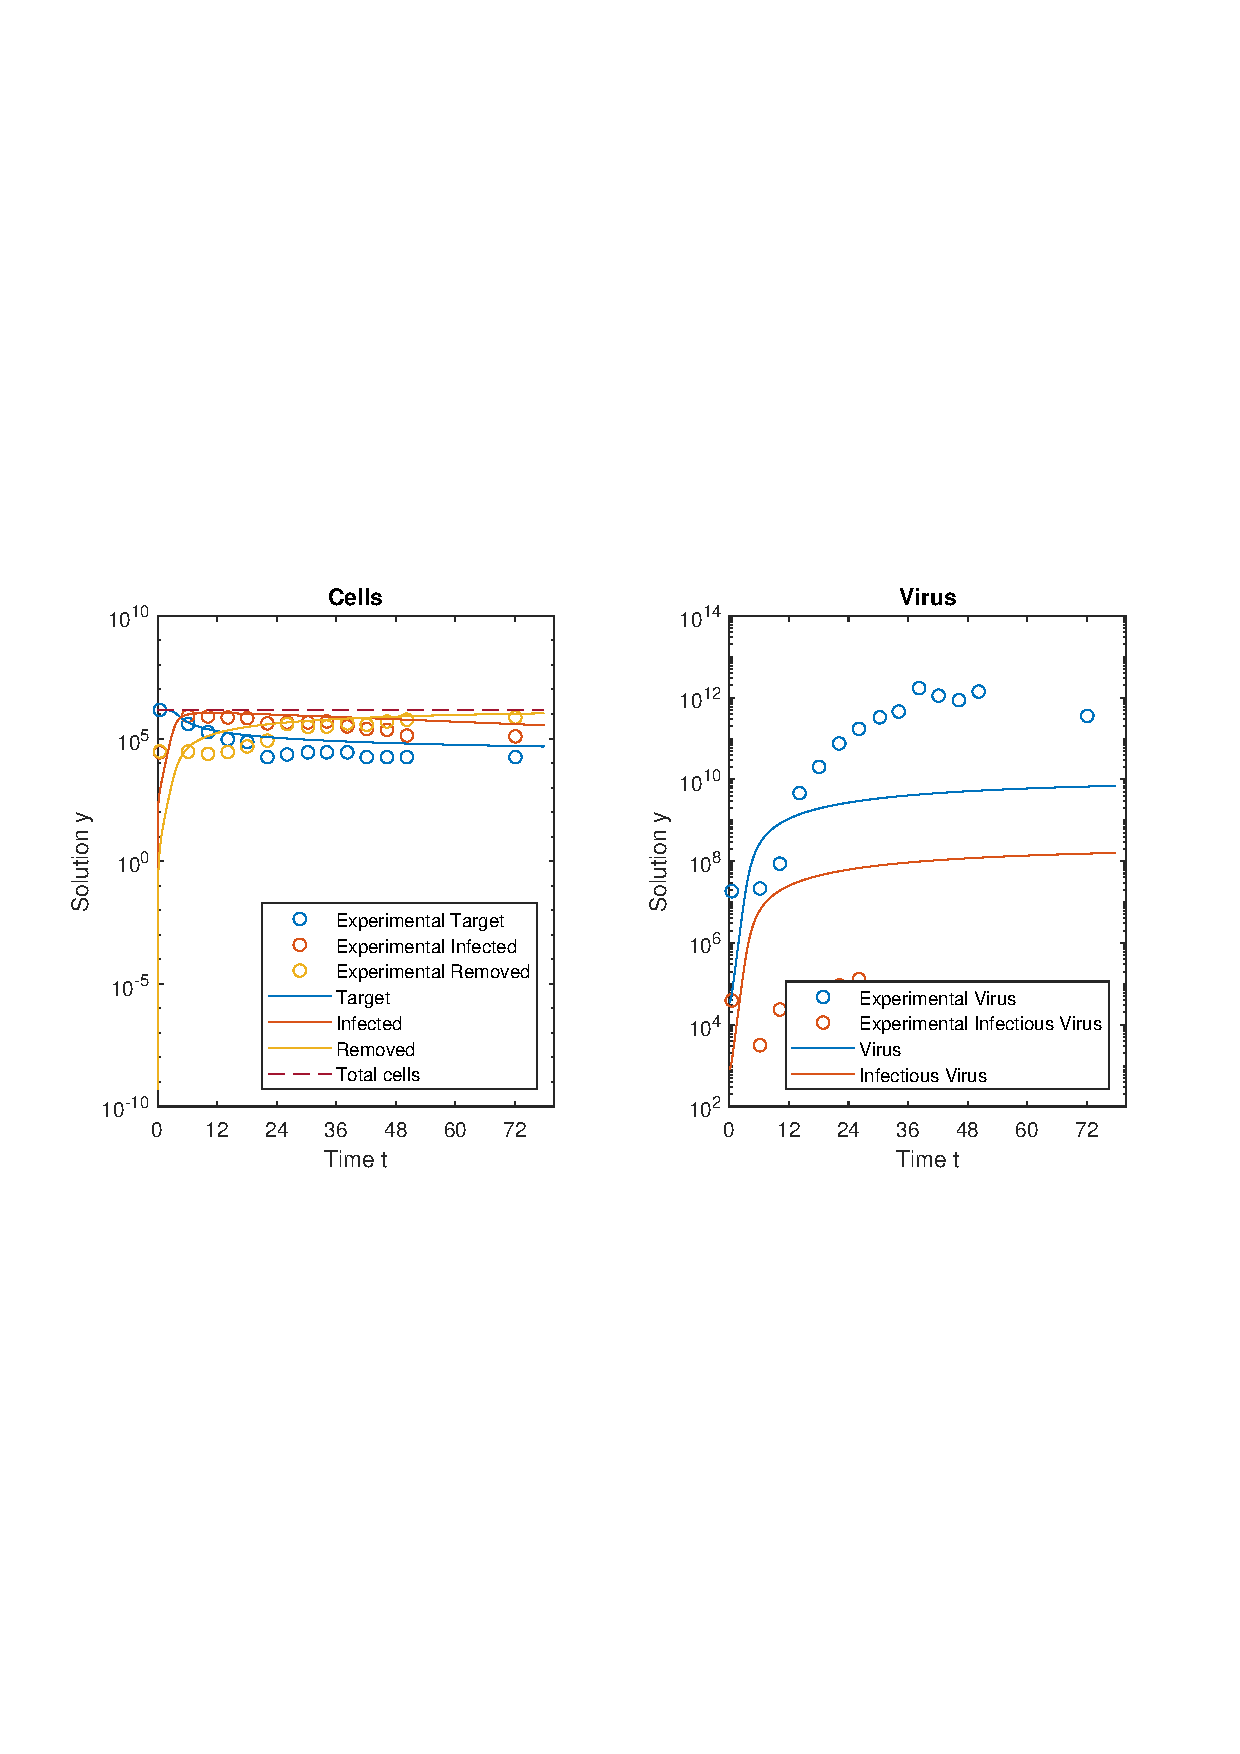
\includegraphics[width=0.55\textwidth, trim={1cm 9.8cm 1cm 9.5cm}, clip]{D_chapters/6_appendix/4_ValidationNIBSC/InfectionDepletionModelTHillIRVViMOI0.025log.pdf}
\caption[T$_{Hill}$IRVV$_i$ model fit for PR/8/34 H1N1 (NIBSC)]%
{T$_{Hill}$IRVV$_i$ model fit PR/8/34 H1N1 (NIBSC)}
\label{figure:THillIRVViValidationNIBSC}
\end{center}
\end{figure}

\begin{figure}[H]
\begin{center}
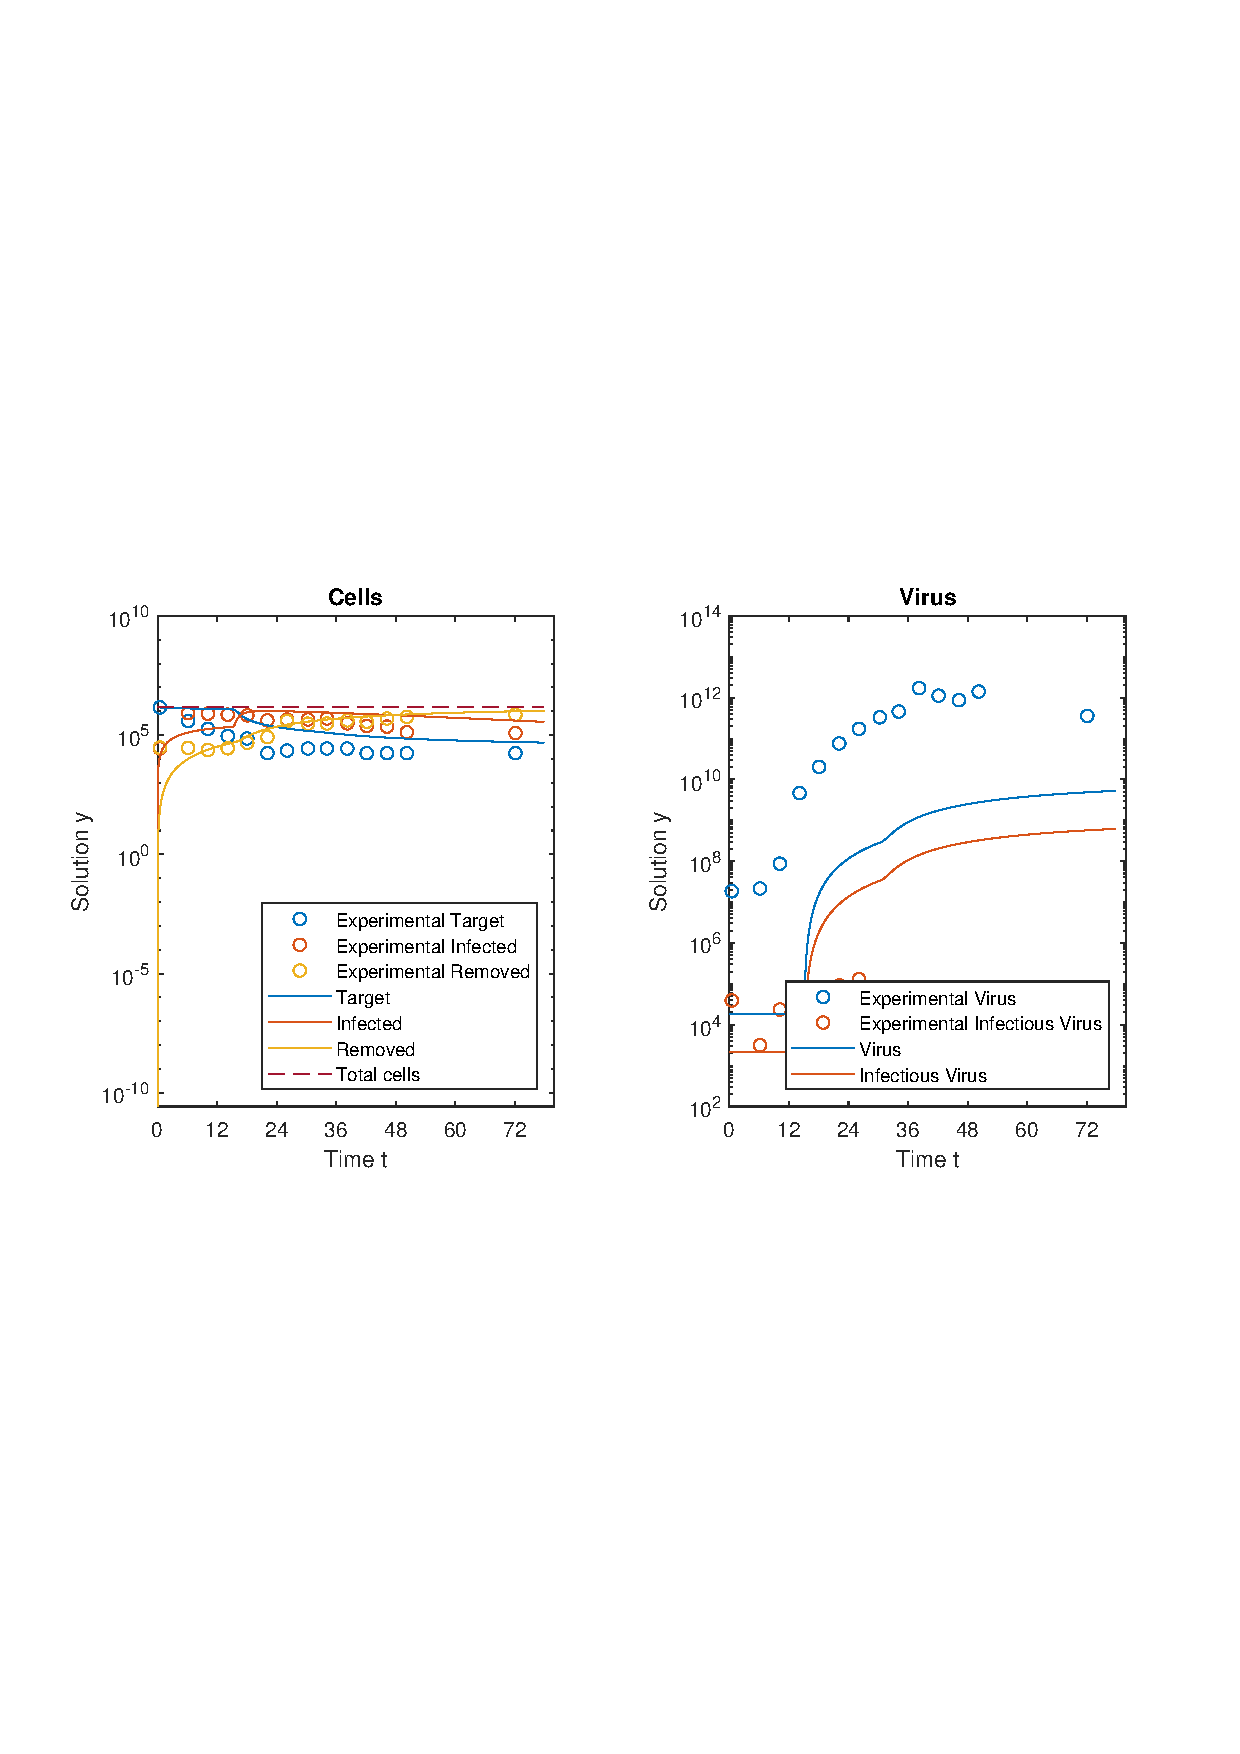
\includegraphics[width=0.55\textwidth, trim={1cm 9.8cm 1cm 9.5cm}, clip]{D_chapters/6_appendix/4_ValidationNIBSC/InfectionDepletionModelTHillIRVViDelayMOI0.025log.pdf}
\caption[T$_{Hill}$IRVV$_i$, delay $\tau = f(\text{MOI})$ model fit forPR/8/34 H1N1 (NIBSC)]%
{T$_{Hill}$IRVV$_i$, delay $\tau = f(\text{MOI})$ model fit for PR/8/34 H1N1 (NIBSC)}
\label{figure:THillIRVViDelayValidationNIBSC}
\end{center}
\end{figure}

\begin{figure}[H]
\begin{center}
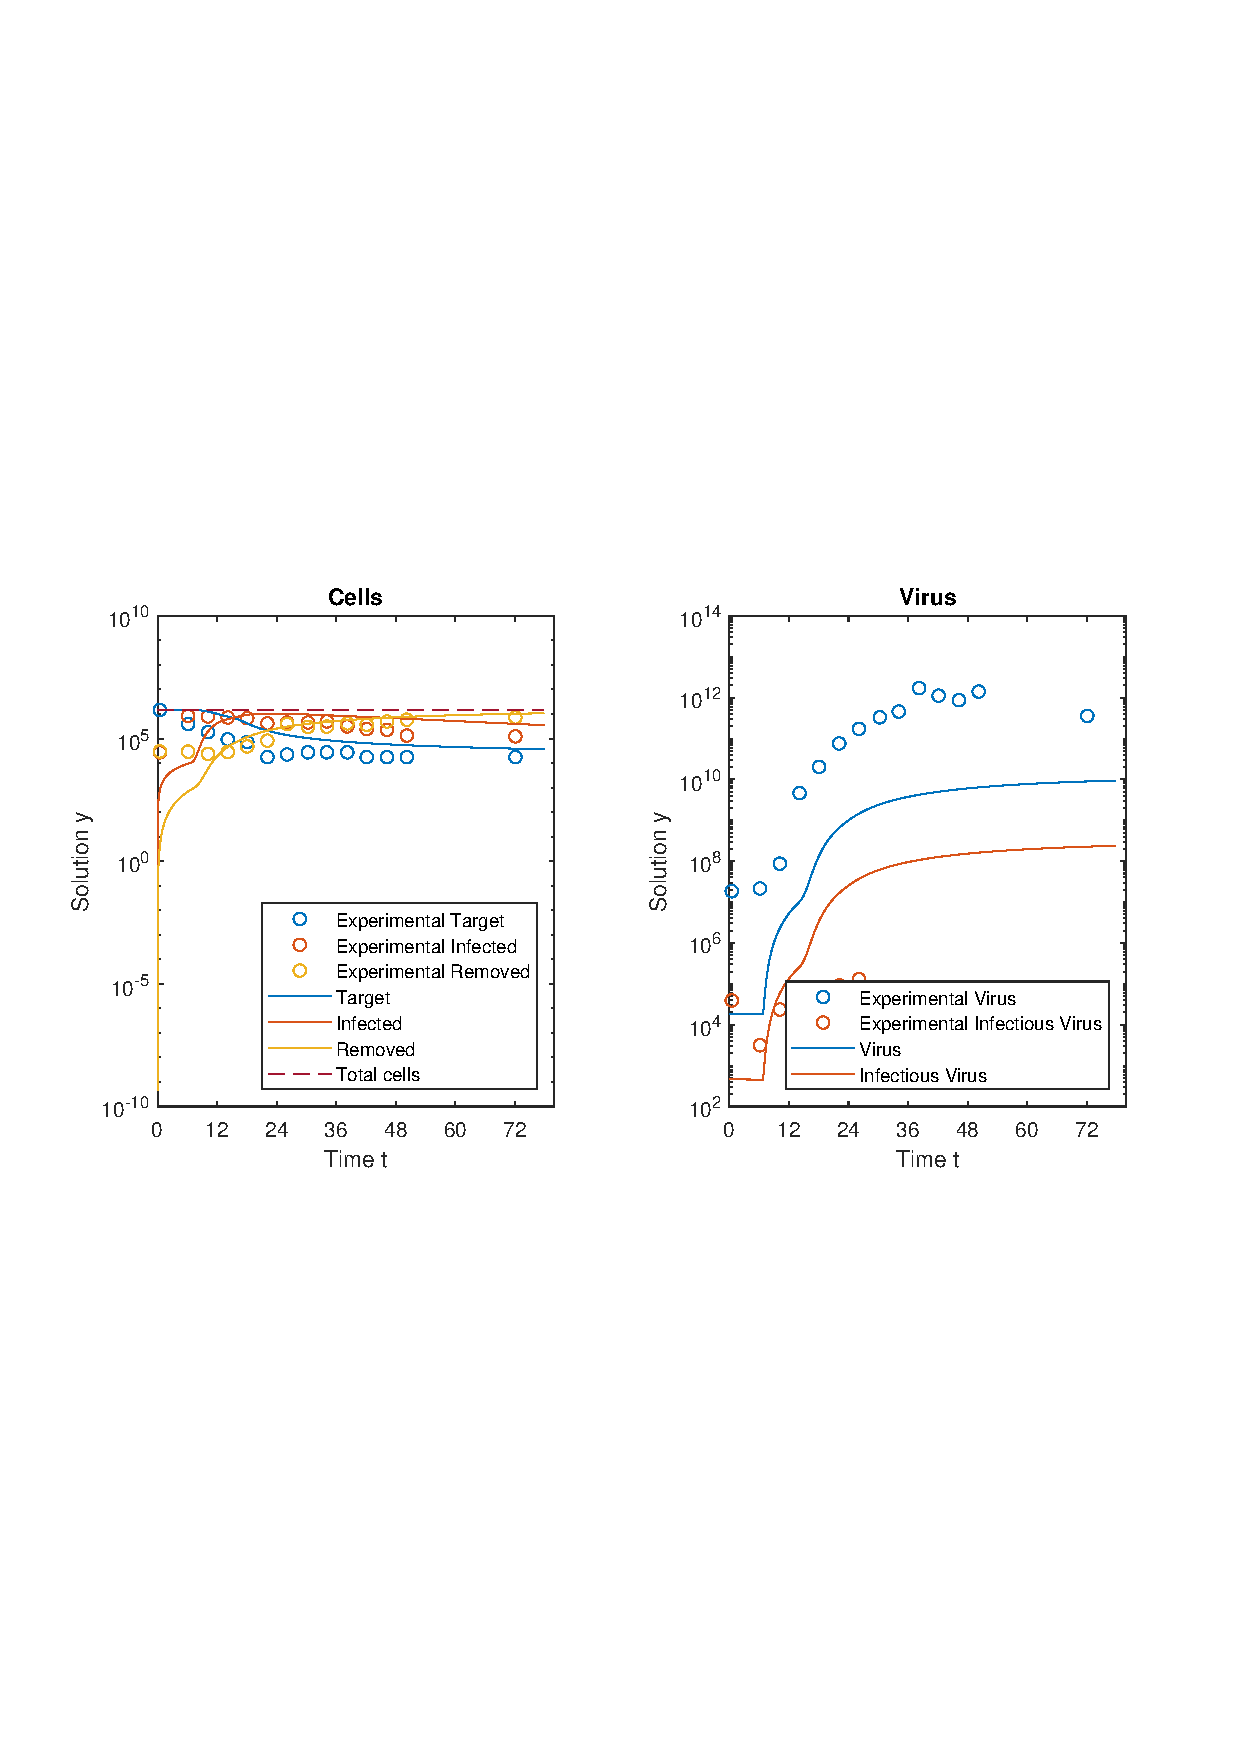
\includegraphics[width=0.55\textwidth, trim={1cm 9.8cm 1cm 9.5cm}, clip]{D_chapters/6_appendix/4_ValidationNIBSC/InfectionDepletionModelTHillIRVViDelayFitTauMOI0.025log.pdf}
\caption[T$_{Hill}$IRVV$_i$, delay $\tau = const$ model fit for PR/8/34 H1N1 (NIBSC)]%
{T$_{Hill}$IRVV$_i$, delay $\tau = const$ model fit for PR/8/34 H1N1 (NIBSC)}
\label{figure:THillIRVViDelayFitTauValidationNIBSC}
\end{center}
\end{figure}

\newpage

\begin{figure}[H]
\begin{center}
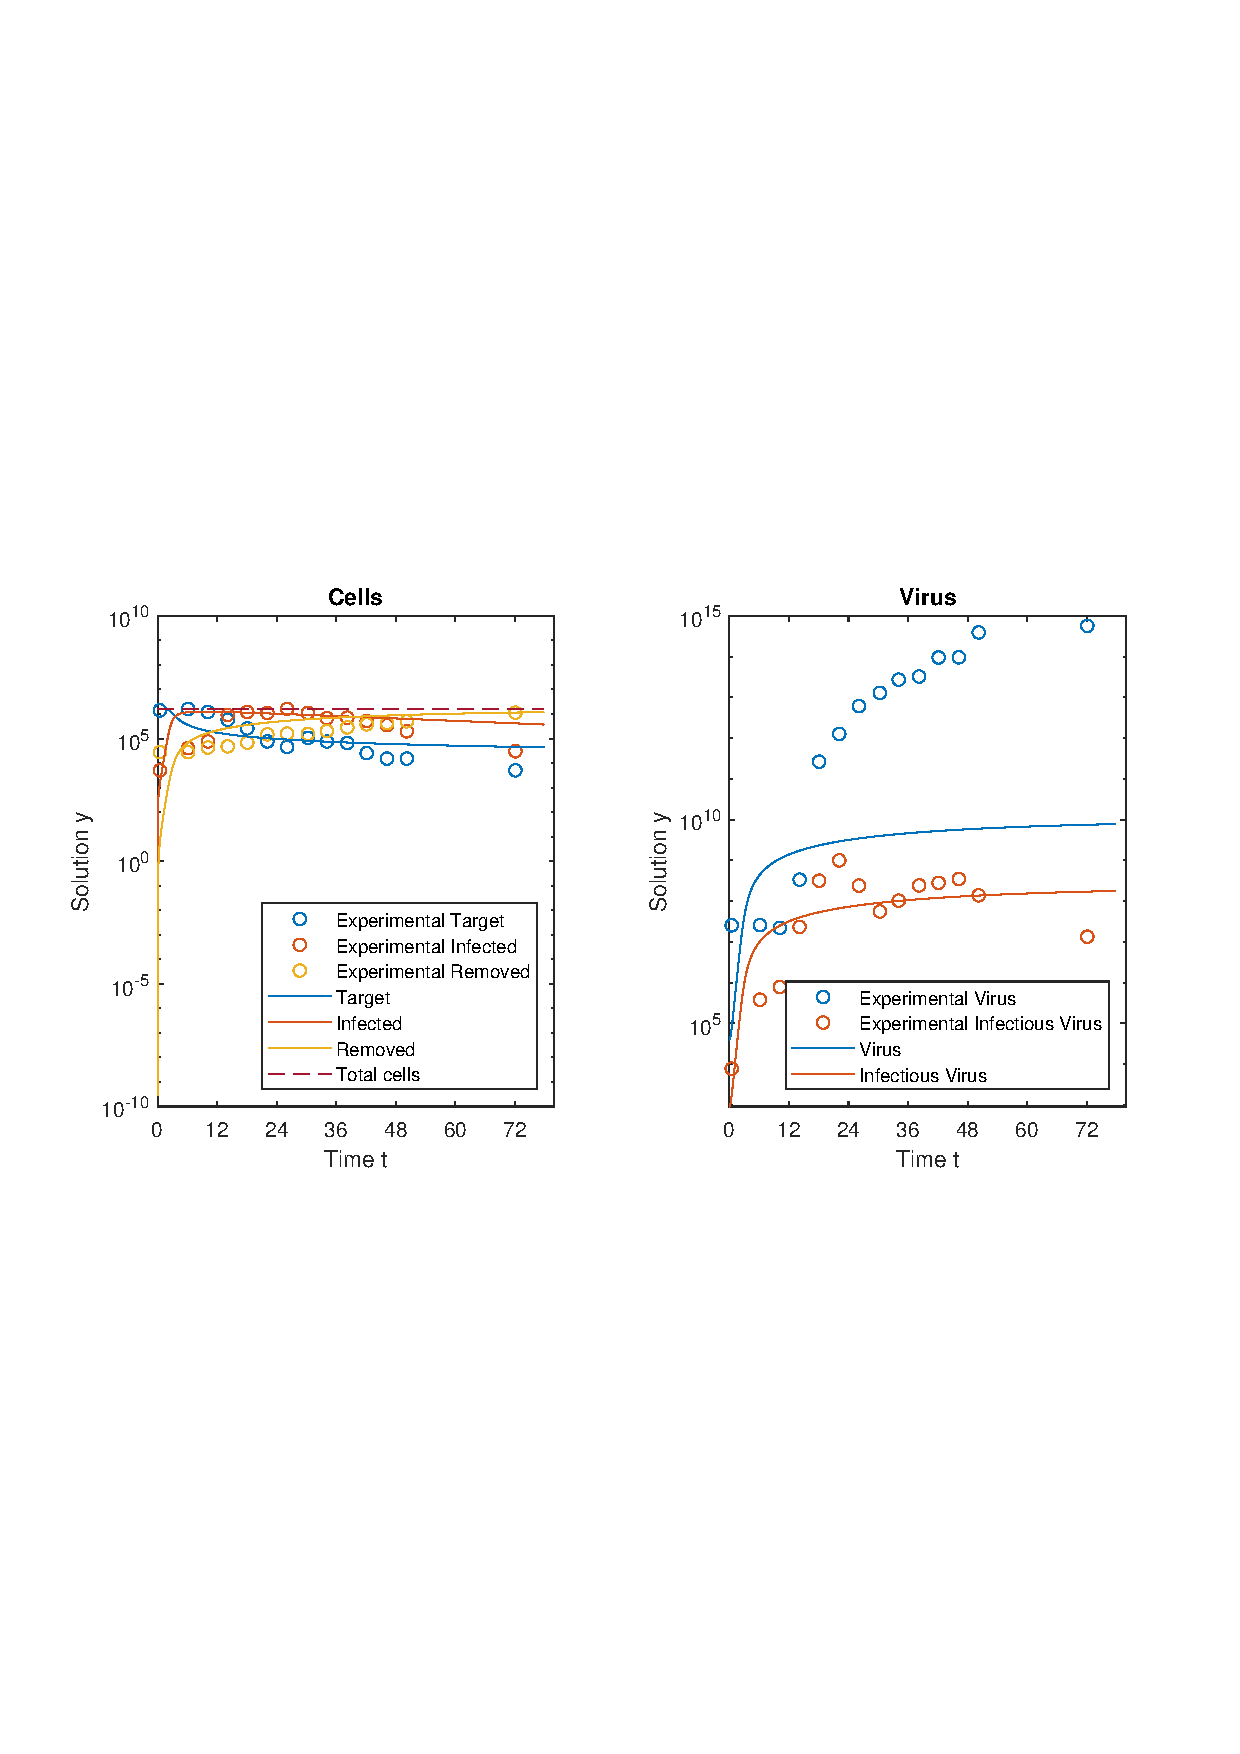
\includegraphics[width=0.55\textwidth, trim={1cm 9.8cm 1cm 9.5cm}, clip]{D_chapters/6_appendix/4_ValidationRKI/InfectionDepletionModelTHillIRVViMOI0.025log.pdf}
\caption[T$_{Hill}$IRVV$_i$ model fit for PR/8/34 H1N1 (RKI)]%
{T$_{Hill}$IRVV$_i$ model fit PR/8/34 H1N1 (RKI)}
\label{figure:THillIRVViValidationRKI}
\end{center}
\end{figure}

\begin{figure}[H]
\begin{center}
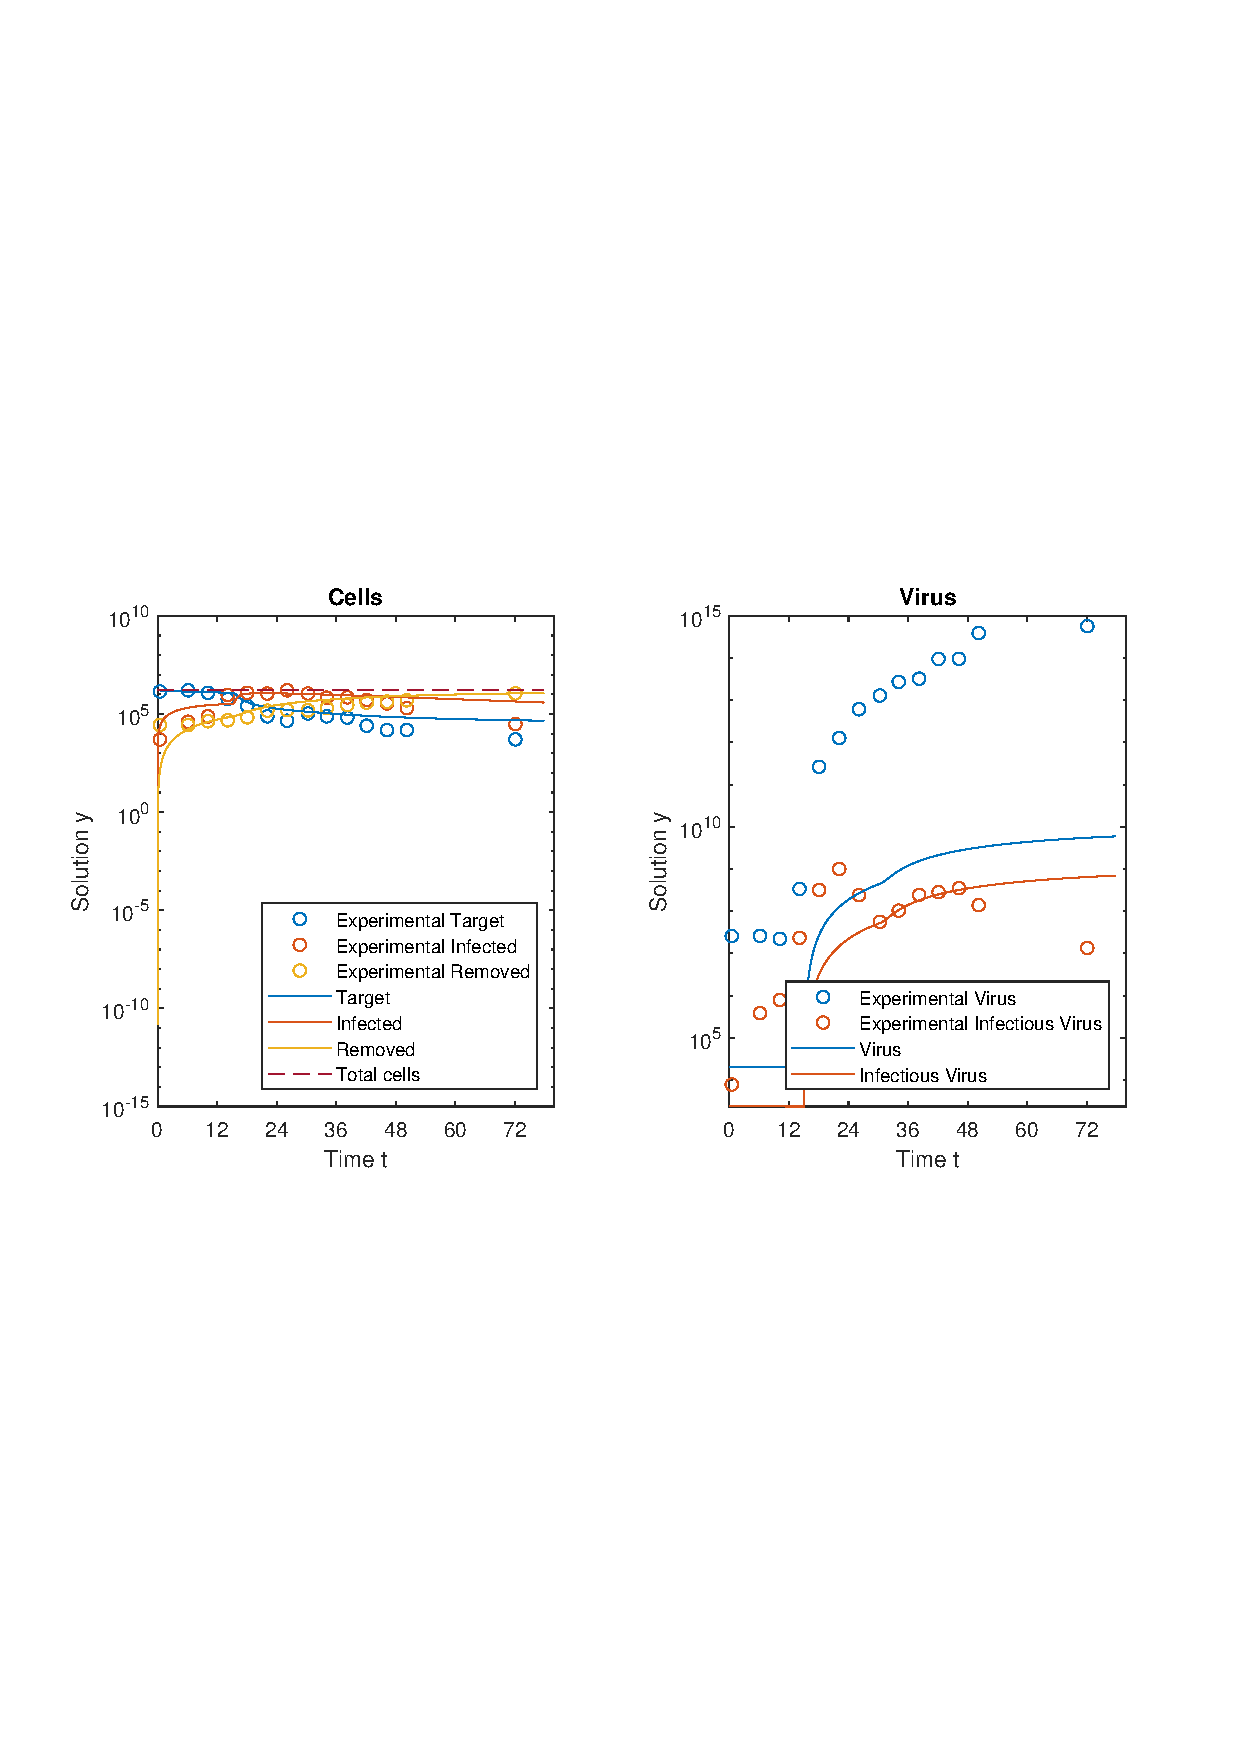
\includegraphics[width=0.55\textwidth, trim={1cm 9.8cm 1cm 9.5cm}, clip]{D_chapters/6_appendix/4_ValidationRKI/InfectionDepletionModelTHillIRVViDelayMOI0.025log.pdf}
\caption[T$_{Hill}$IRVV$_i$, delay $\tau = f(\text{MOI})$ model fit forPR/8/34 H1N1 (RKI)]%
{T$_{Hill}$IRVV$_i$, delay $\tau = f(\text{MOI})$ model fit for PR/8/34 H1N1 (RKI)}
\label{figure:THillIRVViDelayValidationRKI}
\end{center}
\end{figure}

\begin{figure}[H]
\begin{center}
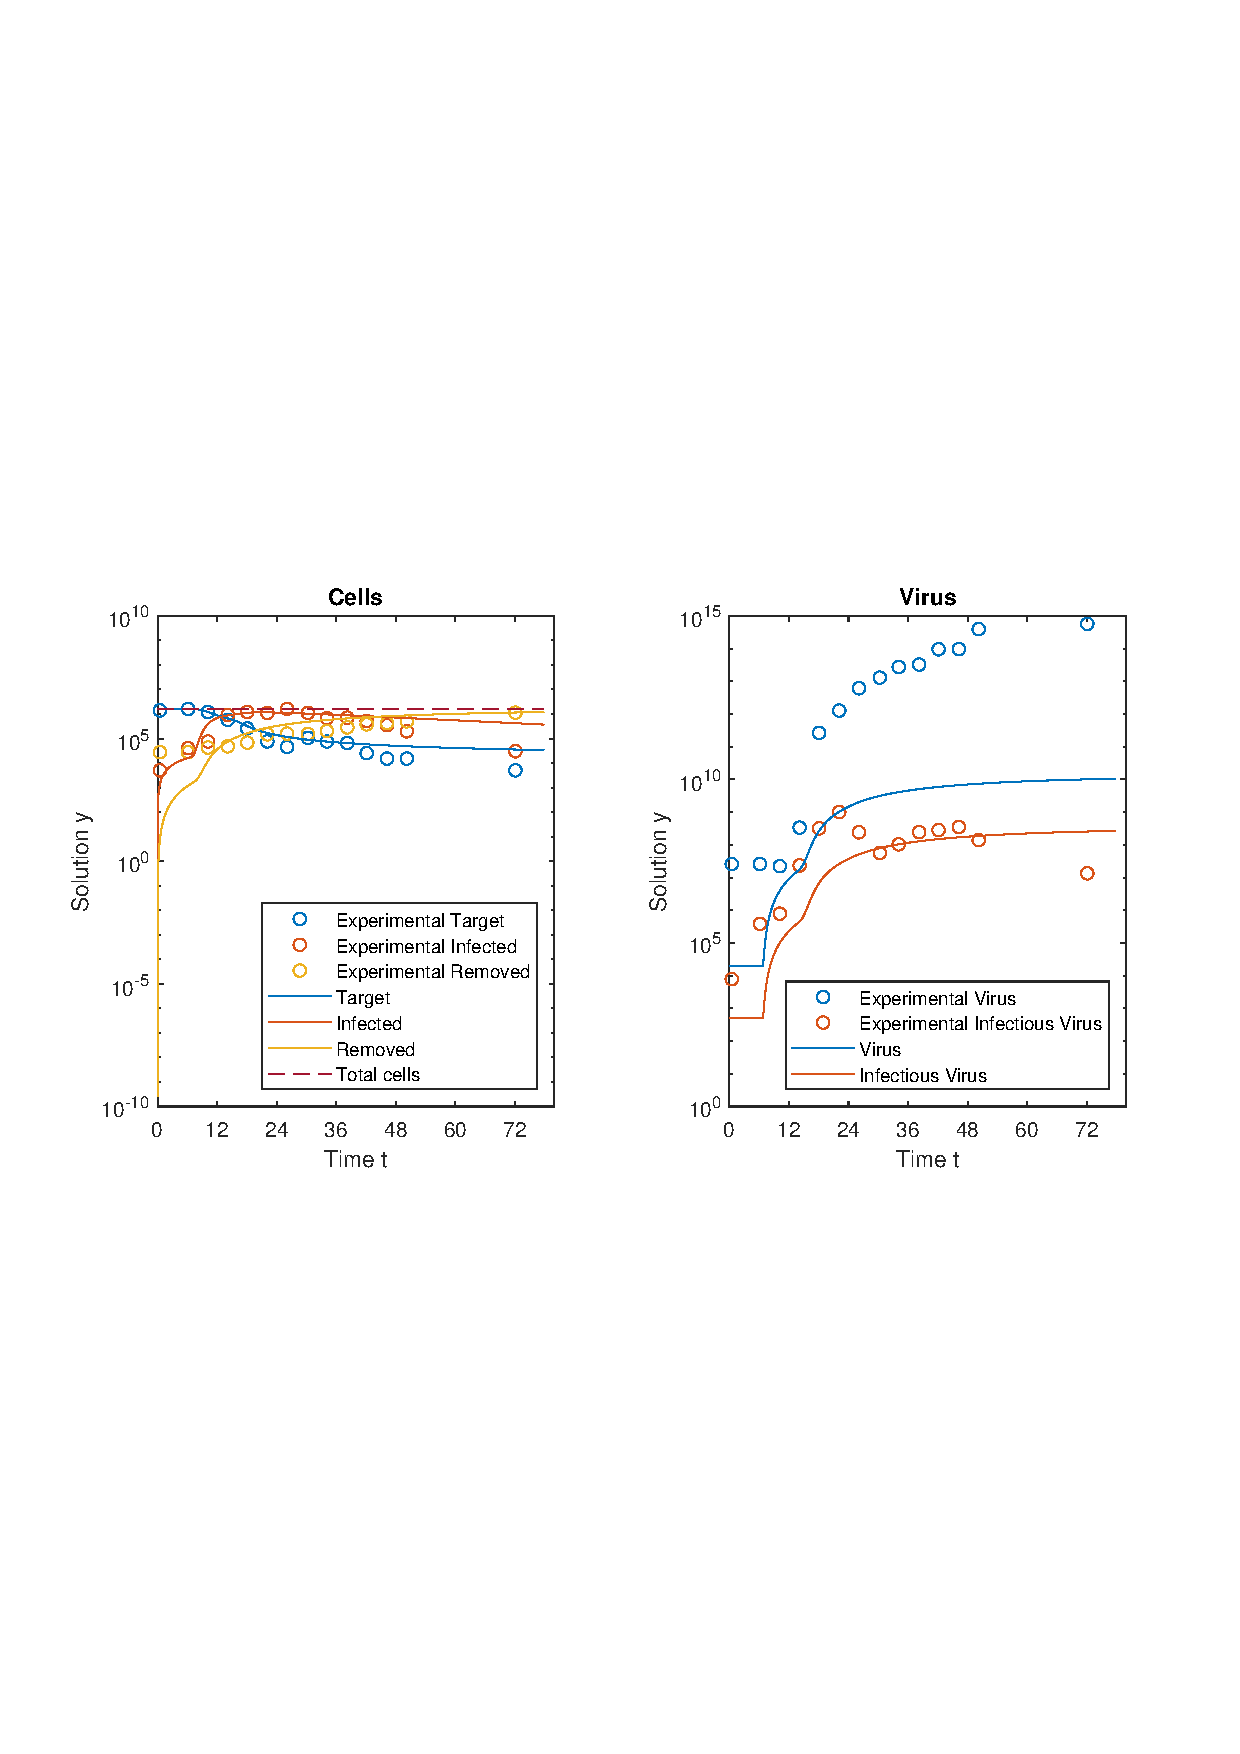
\includegraphics[width=0.55\textwidth, trim={1cm 9.8cm 1cm 9.5cm}, clip]{D_chapters/6_appendix/4_ValidationRKI/InfectionDepletionModelTHillIRVViDelayFitTauMOI0.025log.pdf}
\caption[T$_{Hill}$IRVV$_i$, delay $\tau = const$ model fit for PR/8/34 H1N1 (RKI)]%
{T$_{Hill}$IRVV$_i$, delay $\tau = const$ model fit for PR/8/34 H1N1 (RKI)}
\label{figure:THillIRVViDelayFitTauValidationRKI}
\end{center}
\end{figure}

\newpage

\begin{figure}[H]
\begin{center}
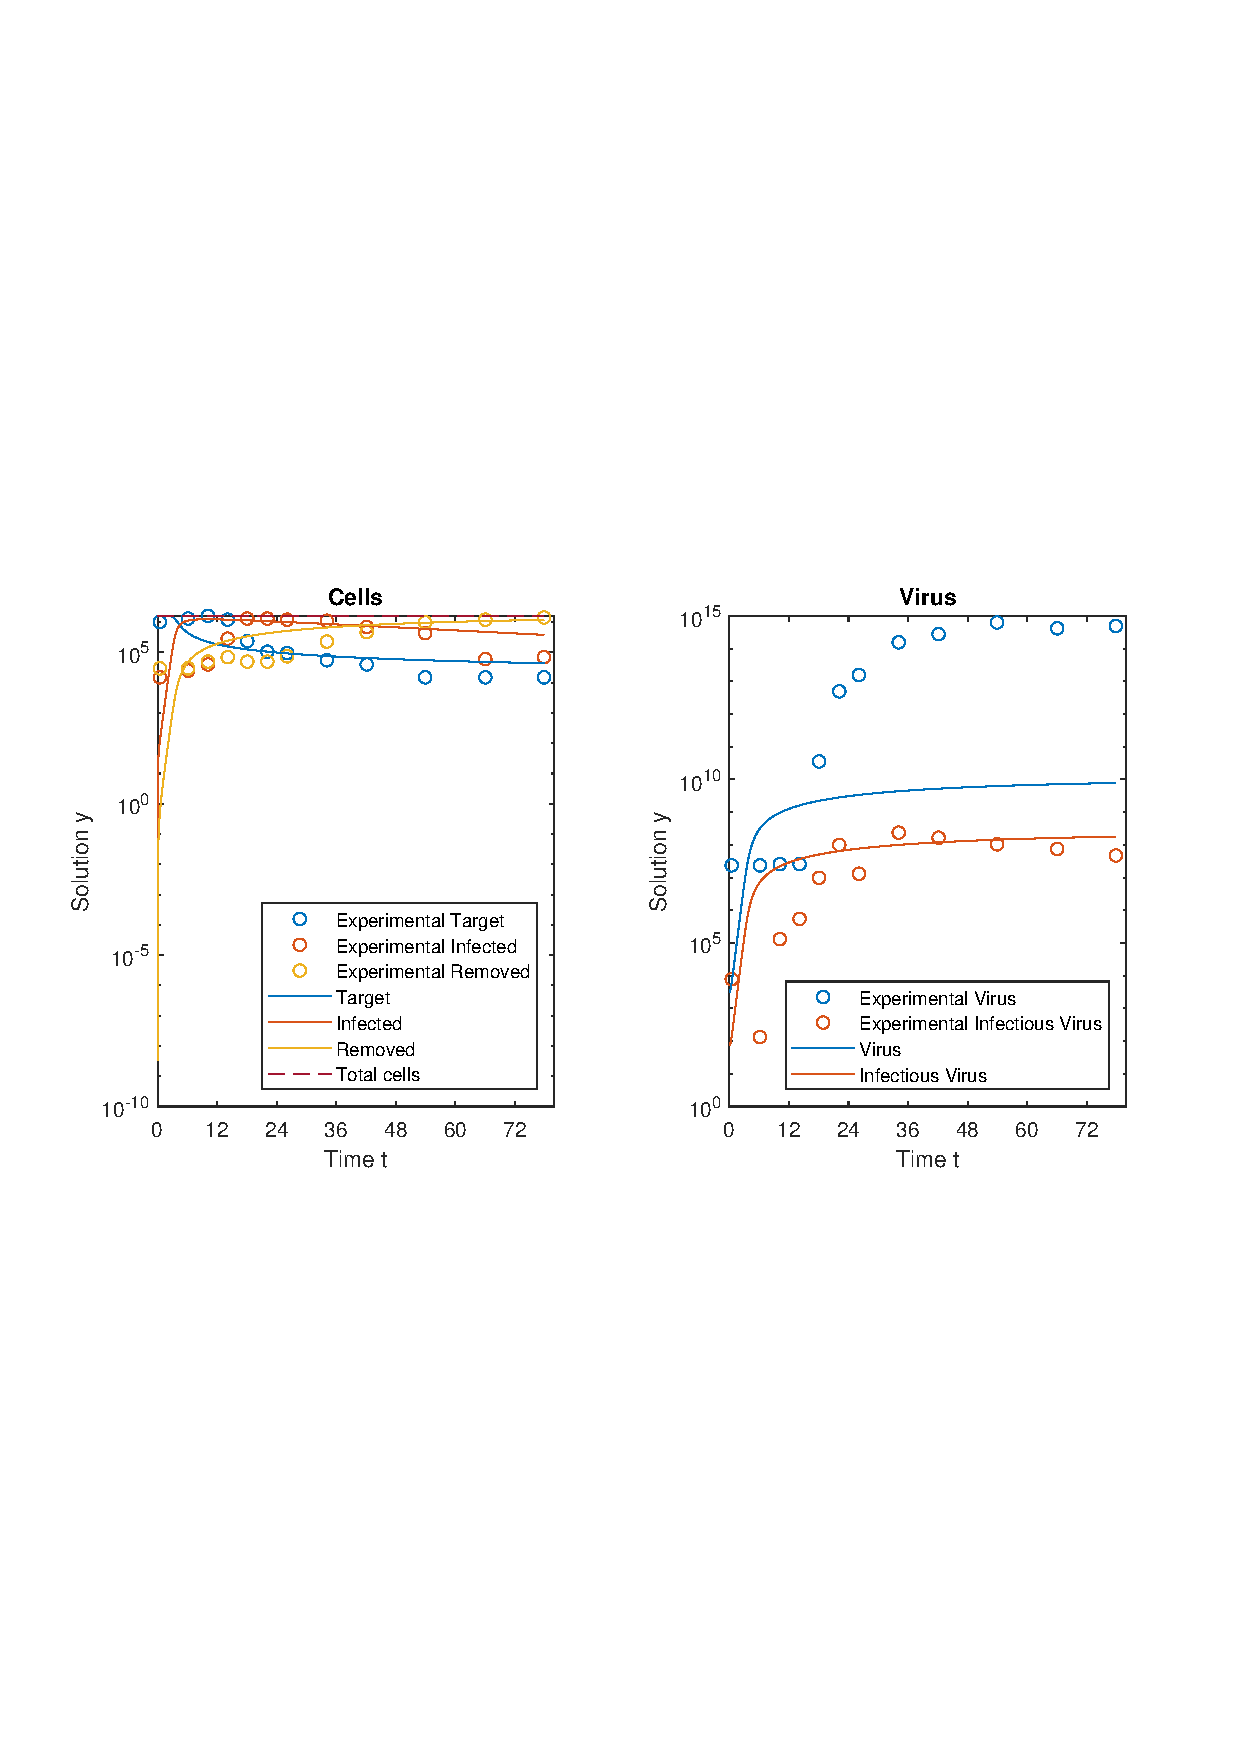
\includegraphics[width=0.55\textwidth, trim={1cm 9.8cm 1cm 9.5cm}, clip]{D_chapters/6_appendix/4_ValidationH3N2/InfectionDepletionModelTHillIRVViMOI0.002log.pdf}
\caption[T$_{Hill}$IRVV$_i$ model fit for WSN/67/2005 HGR H3N2]%
{T$_{Hill}$IRVV$_i$ model fit WSN/67/2005 HGR H3N2}
\label{figure:THillIRVViValidationRKI}
\end{center}
\end{figure}

\begin{figure}[H]
\begin{center}
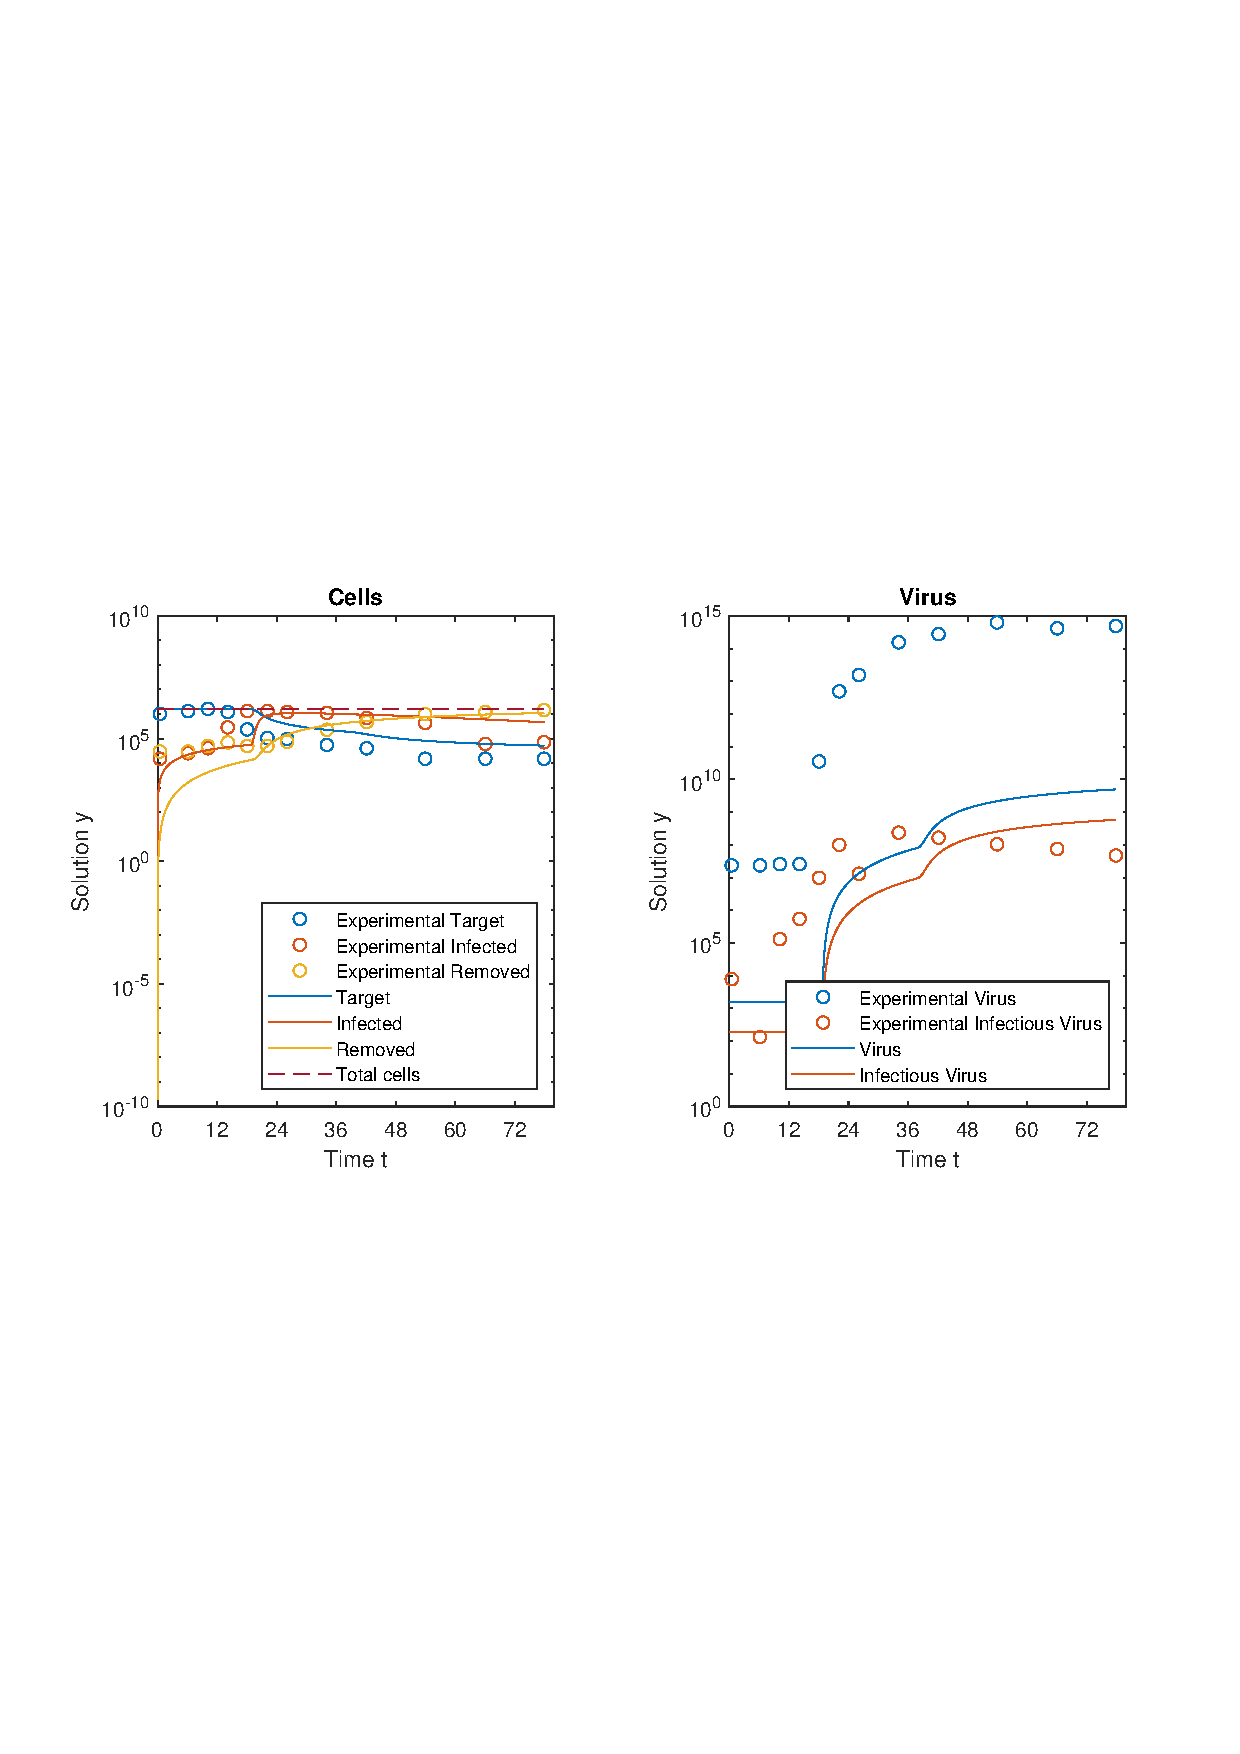
\includegraphics[width=0.55\textwidth, trim={1cm 9.8cm 1cm 9.5cm}, clip]{D_chapters/6_appendix/4_ValidationH3N2/InfectionDepletionModelTHillIRVViDelayMOI0.002log.pdf}
\caption[T$_{Hill}$IRVV$_i$, delay $\tau = f(\text{MOI})$ model fit for WSN/67/2005 HGR H3N2]%
{T$_{Hill}$IRVV$_i$, delay $\tau = f(\text{MOI})$ model fit for WSN/67/2005 HGR H3N2}
\label{figure:THillIRVViDelayValidationRKI}
\end{center}
\end{figure}

\begin{figure}[H]
\begin{center}
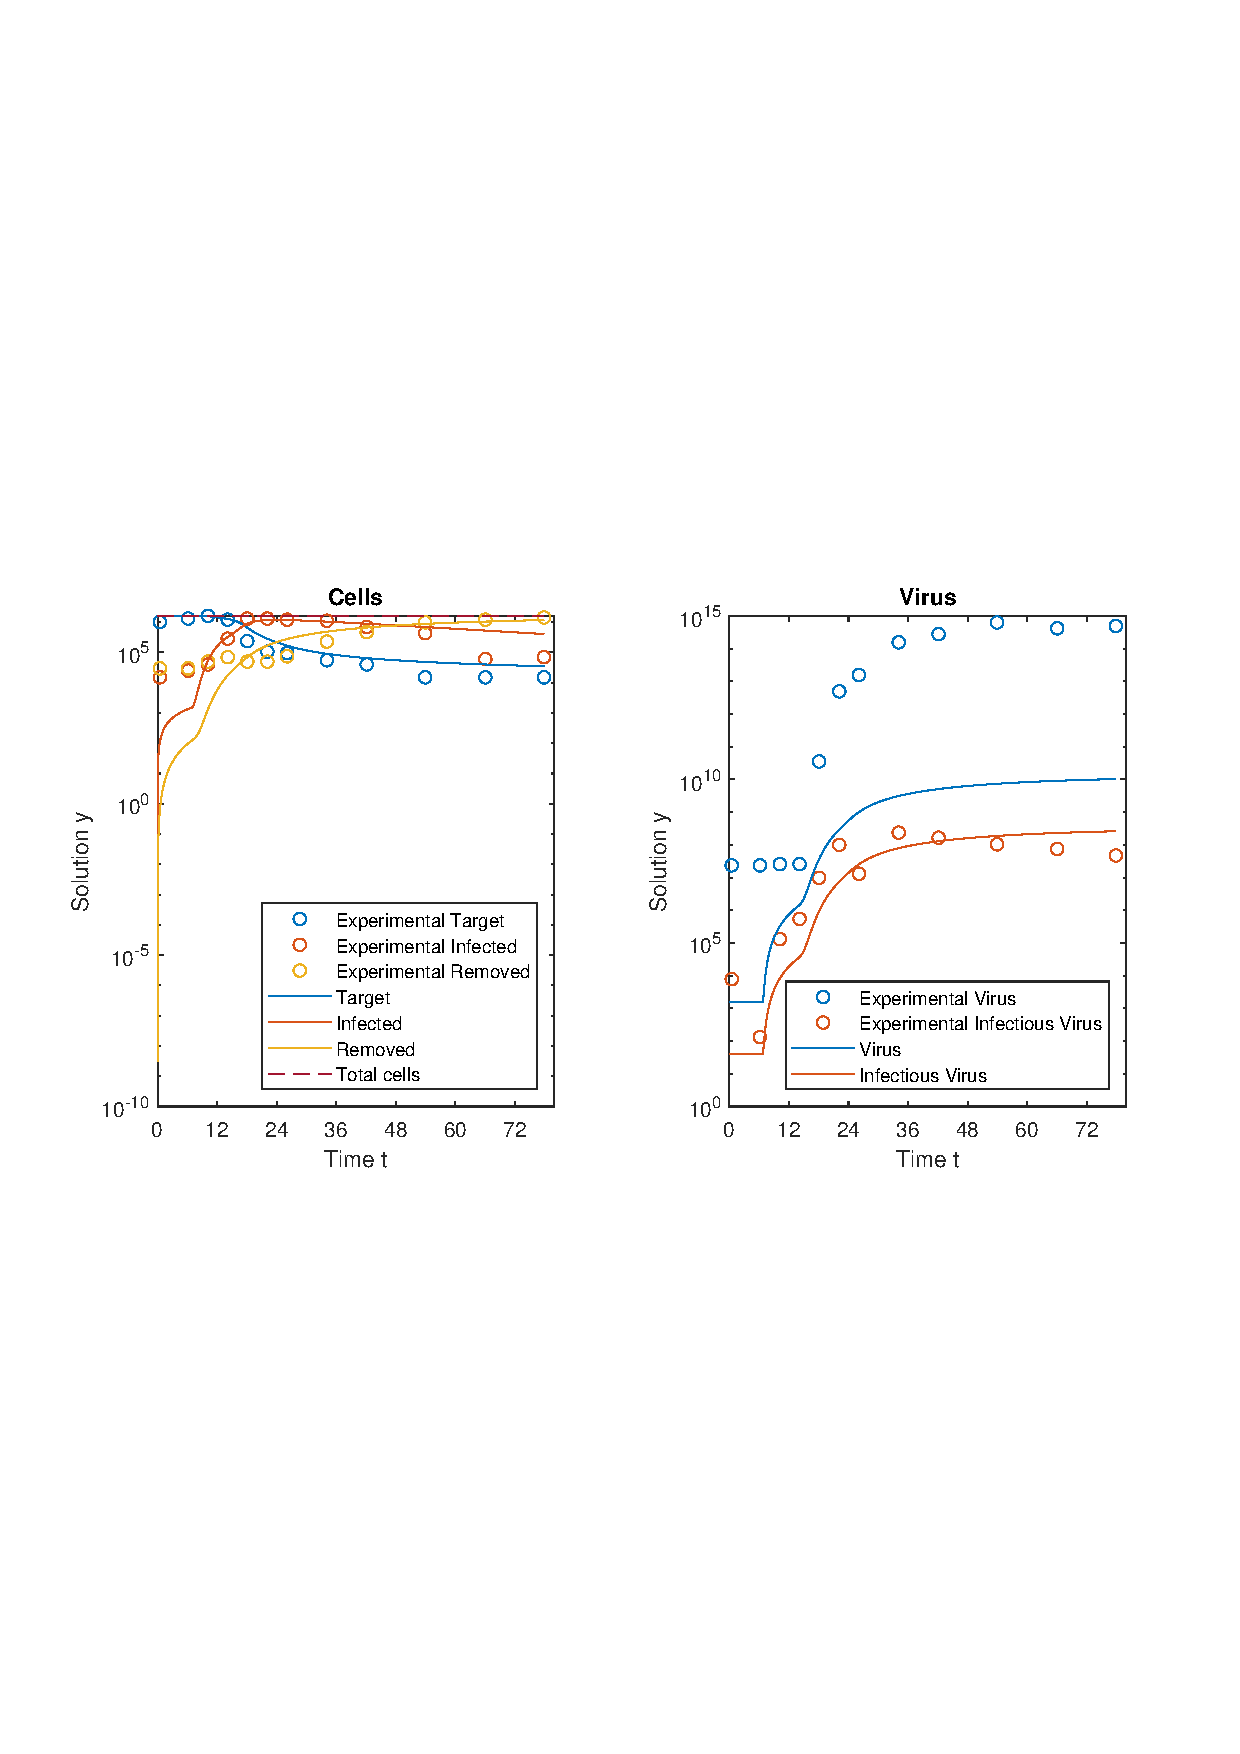
\includegraphics[width=0.55\textwidth, trim={1cm 9.8cm 1cm 9.5cm}, clip]{D_chapters/6_appendix/4_ValidationH3N2/InfectionDepletionModelTHillIRVViDelayFitTauMOI0.002log.pdf}
\caption[T$_{Hill}$IRVV$_i$, delay $\tau = const$ model fit for WSN/67/2005 HGR H3N2]%
{T$_{Hill}$IRVV$_i$, delay $\tau = const$ model fit for WSN/67/2005 HGR H3N2}
\label{figure:THillIRVViDelayFitTauValidationRKI}
\end{center}
\end{figure}